\documentclass[tikz,border=5pt]{standalone}
\usepackage{luatexja}
\usepackage[hiragino-pron]{luatexja-preset}
\usepackage{amsmath,amssymb}
\usepackage{pgfplots}
\pgfplotsset{compat=1.18}
\usetikzlibrary{arrows.meta,calc,decorations.markings,patterns,positioning}

% Common styles
\tikzset{
  axis/.style={-{Stealth[length=6pt]}, thick},
  curve/.style={thick, red},
  dashed curve/.style={thick, dashed, blue},
  dot/.style={circle, fill, inner sep=1.5pt},
  open dot/.style={circle, draw, fill=white, inner sep=1.5pt},
}

\begin{document}
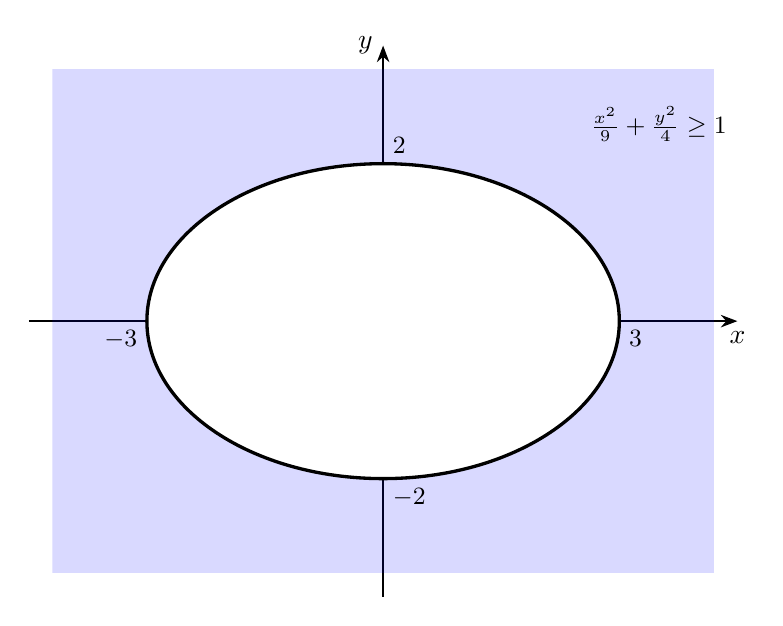
\begin{tikzpicture}
  % Axes
  \draw[axis] (-4.5,0) -- (4.5,0) node[below] {$x$};
  \draw[axis] (0,-3.5) -- (0,3.5) node[left] {$y$};

  % Fill exterior region
  \begin{scope}
    \clip (-4.2,-3.2) rectangle (4.2,3.2);
    \fill[blue, opacity=0.15] (-4.2,-3.2) rectangle (4.2,3.2);
    % Cut out interior of ellipse
    \fill[white] (0,0) ellipse (3 and 2);
  \end{scope}

  % Ellipse boundary (included, very thick black)
  \draw[very thick] (0,0) ellipse (3 and 2);

  % Labels
  \node[below right, font=\small] at (3,0) {$3$};
  \node[below left, font=\small] at (-3,0) {$-3$};
  \node[above right, font=\small] at (0,2) {$2$};
  \node[below right, font=\small] at (0,-2) {$-2$};
  \node[font=\small] at (3.5,2.5) {$\frac{x^2}{9}+\frac{y^2}{4} \geq 1$};
\end{tikzpicture}
\end{document}
